\documentclass{article}

\usepackage{apacite}
\usepackage[table,xcdraw]{xcolor} % Color the table
\usepackage{parskip} % Disable the second and onward paragraph indentation
\usepackage{listings} % Code Snippets
\lstset{language=Python}
\usepackage{float} % \begin{table}[H] To avoid table repositioning
\usepackage{graphicx} % Insert images
\usepackage{subcaption}
\graphicspath{ {./Plots/} }

\renewcommand{\arraystretch}{1.5} 		% Adjust rows' height in table

\title	{Alberi Binari di Ricerca vs Alberi Rosso Neri}
\author	{Marco De Groskovskaja}
\date	{\today}

\usepackage [
	a4paper,
	left=3cm,
	right=3cm,
	top=3cm,
	bottom=3cm,
] {geometry}

\begin{document}
	\maketitle
	
	\section{Introduzione}
	
	L'albero binario di ricerca (BST) e l' albero rosso-nero (RBT) sono due importanti strutture di dati utilizzate per organizzare e gestire informazioni. Entrambi sono alberi binari, ma differiscono nella loro complessità e nei vantaggi che offrono. Questa relazione esplora le differenze di complessità tra i due alberi e valuta l'efficienza delle loro operazioni di inserimento, ricerca e cancellazione. L'obiettivo è di fornire una comprensione approfondita delle prestazioni dei due alberi.
	
	\section{Albero Binario di Ricerca}
	
		\subsection{Definizione}
		
			Un albero binario di ricerca è un albero binario per il quale valgono le seguenti proprietà:
		
			\begin{enumerate}
				\item Per ogni nodo dell'albero, il valore del nodo è maggiore del valore di ciascun nodo del suo sotto-albero sinistro.
				\item Per ogni nodo dell'albero, il valore del nodo è minore del valore di ciascun nodo del suo sotto-albero destro.
			\end{enumerate}

		\subsection{Definizione della struttura dati}
			La struttura dati dell' albero binario di ricerca è così definita:

			\begin{lstlisting}
	class BinarySearchTree:
		class Node:
			parent
			left
			right
			data
		null
		root
			\end{lstlisting}

		\subsection{Implementazione software}
			L'implementazione dell'albero binario di ricerca è descritta nei file Python \textbf{\textit{BinarySearchTree.py}} e \textbf{\textit{\_BinarySearchTree.py}} alla relazione allegati.
			
			I seguenti metodi sono stati definiti e implementati:
			\newline
			\colorbox{lightgray}{inorder\_walk()} \colorbox{lightgray}{preorder\_walk()} \colorbox{lightgray}{postorder\_walk()} \colorbox{lightgray}{insert(data)} \colorbox{lightgray}{transplant(rm\_tree\_root, ins\_tree\_root)} \colorbox{lightgray}{remove(data)} \colorbox{lightgray}{search(data)} \colorbox{lightgray}{min()} \colorbox{lightgray}{max()} \colorbox{lightgray}{successor(node)} \colorbox{lightgray}{predecessor(node)}.
			
		%\newpage
		\subsection{Complessità Algoritmica}
			I limiti asintotici delle complessità temporale e spaziale previste per le operazione di ricerca, inserimento e cancellazione sono descritti nella seguente tabella:
			
			\begin{table}[ht]
				\centering
				\begin{tabular}{|l|ccc|}
					\rowcolor[HTML]{C0C0C0}
					\hline
					Operazione    & Caso Peggiore & Caso Medio & Caso Migliore \\
					\hline
					Ricerca       & O(n)          & O(log n)    & O(1)          \\
					\hline
					Inserimento   & O(n)          & O(log n)    & O(1)          \\
					\hline
					Cancellazione & O(n)          & O(log n)    & O(1)		   \\
					\hline
					\noalign{\smallskip}
					\noalign{\smallskip}
					\hline
					Spazio		  &			 	  & O(n) 	   &			   \\
					\hline
				\end{tabular}
				\caption{Complessità Temporale e Spaziale dell' Albero Rosso Nero}
			\end{table}

	\newpage
	\section{Albero Rosso Nero}

		\subsection{Definizione}
		
			Un albero rosso nero è un albero binario di ricerca per il quale valgono le seguenti proprietà:

			\begin{enumerate}
				\item Ogni nodo dell'albero ha un colore che può essere rosso o nero.
				\item La radice dell'albero è di colore nero.
				\item Se un nodo dell'albero è di colore rosso, allora entrambi i suoi figli sono di colore nero.
				\item Tutte le foglie dell'albero hanno valore nullo e sono di colore nero
				\item Tutti i cammini da ogni nodo dell'albero alle foglie, contengono lo stesso numero di nodi neri.
			\end{enumerate}
		
		\subsection{Definizione della struttura dati}
			La struttura dati dell' albero rosso nero estende la struttura dati dell' albero binario di ricerca, aggiungendo l'attributo del nodo  \colorbox{lightgray}{color}:
			\begin{lstlisting}
	class BinarySearchTree:
		class Node:
			parent
			left
			right
			data
			color
		null
		root
			\end{lstlisting}
		
		\subsection{Implementazione software}
			L'implementazione dell'albero rosso nero è descritta nei file Python \textbf{\textit{RedBlackTree.py}}, \textbf{\textit{\_RedBlackTree.py}}, \textbf{\textit{BinarySearchTree.py}}, \textbf{\textit{\_BinarySearchTree.py}} alla relazione allegati.
			
			L'implementazione dell' albero rosso nero di fatto non è altro che un estensione dell' albero binario di ricerca a cui si aggiungo e/o sovrascrivono attributi o metodi.
			
			I seguenti metodi sono ereditati dall' implementazione dell' albero binario di ricerca:
			\newline
			\colorbox{lightgray}{inorder\_walk()} \colorbox{lightgray}{preorder\_walk()} \colorbox{lightgray}{postorder\_walk()} \colorbox{lightgray}{transplant(rm\_tree\_root, ins\_tree\_root)} \colorbox{lightgray}{search(data)} \colorbox{lightgray}{min()} \colorbox{lightgray}{max()} \colorbox{lightgray}{successor(node)} \colorbox{lightgray}{predecessor(node)}.
			
			I seguenti metodi sono stati sovrascritti:
			\colorbox{lightgray}{insert(data)} \colorbox{lightgray}{remove(data)}
			
			I seguenti metodi sono stati implementati: \colorbox{lightgray}{left\_rotate(node)} \colorbox{lightgray}{right\_rotate(node)}
			
		\newpage
		\subsection{Complessità Algoritmica}

				I limiti asintotici delle complessità temporale e spaziale previste per le operazione di ricerca, inserimento e cancellazione sono descritti nella seguente tabella:
	
				\begin{table}[ht]
					\centering
					\begin{tabular}{|l|ccc|}
						\rowcolor[HTML]{C0C0C0}
						\hline
						Operazione    & Caso Peggiore & Caso Medio & Caso Migliore \\
						\hline
						Ricerca       & O(log n)          & O(log n)    & O(1)          \\
						\hline
						Inserimento   & O(log n)          & O(log n)    & O(1)          \\
						\hline
						Cancellazione & O(log n)          & O(log n)    & O(1)		   \\
						\hline
						\noalign{\smallskip}
						\noalign{\smallskip}
						\hline
						Spazio		  &			 	  & O(n) 	   &			   \\
						\hline
					\end{tabular}
					\caption{Complessità Temporale e Spaziale dell' Albero Rosso Nero}
				\end{table}

	\section{Test sulle operazioni}
		Di seguito vengono riportati i grafici eseguiti sull'implementazione software dell' albero binario di ricerca e dell' albero rosso nero, attraverso l' unità di testing definita nel file Python \colorbox{lightgray}{TestUnit.py} ed eseguita da \colorbox{lightgray}{main.py} per le operazioni di inserimento, ricerca e cancellazione.
		
		I test sono stati eseguiti sia per sequenze in input \textit{Randomized} che sequenze in input \textit{Unbalanced}.
		
		\newpage
		\subsection{Operazioni su BST}
		
			\begin{figure}[h!]
				\centering
				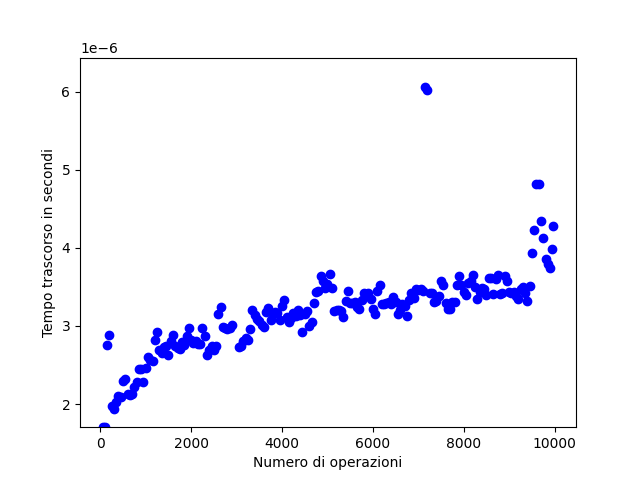
\includegraphics[scale = 0.8]{BST_Insertions}
				\caption{Inserimenti \textit{input randomizzato}}
			\end{figure}
			\begin{figure}[h!]
				\centering
				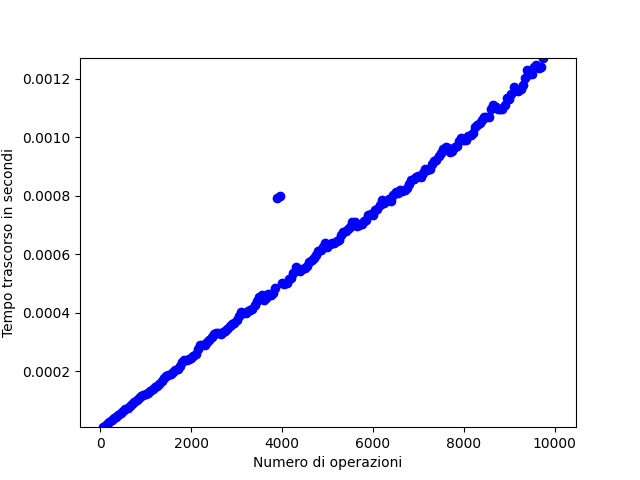
\includegraphics[scale = 0.8]{BST_Unbalanced_Insertions}
				\caption{Inserimenti \textit{input non bilanciato}}
			\end{figure}
			\begin{figure}[h!]
				\centering
				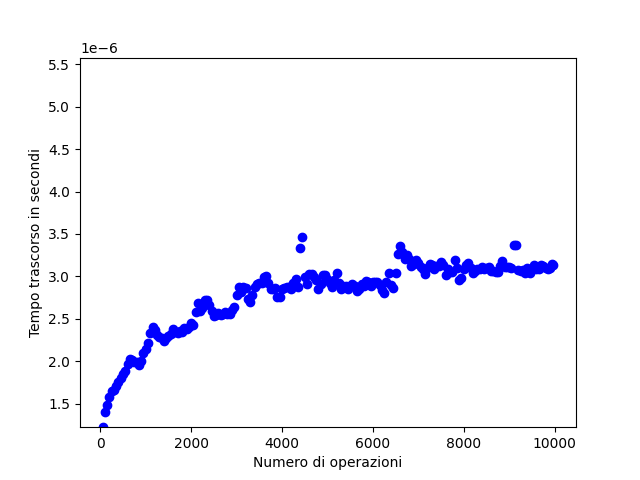
\includegraphics[scale = 0.8]{BST_Searches}
				\caption{Ricerche \textit{input randomizzato}}
			\end{figure}
			\begin{figure}[h!]
				\centering
				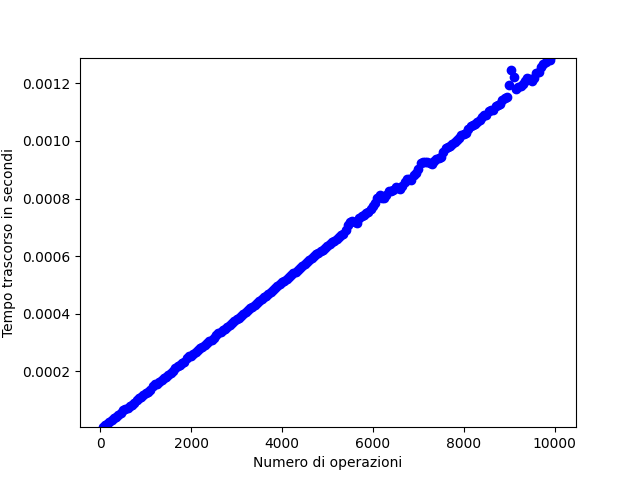
\includegraphics[scale = 0.8]{BST_Unbalanced_Searches}
				\caption{Ricerche \textit{input non bilanciato}}
			\end{figure}
			\begin{figure}[h!]
				\centering
				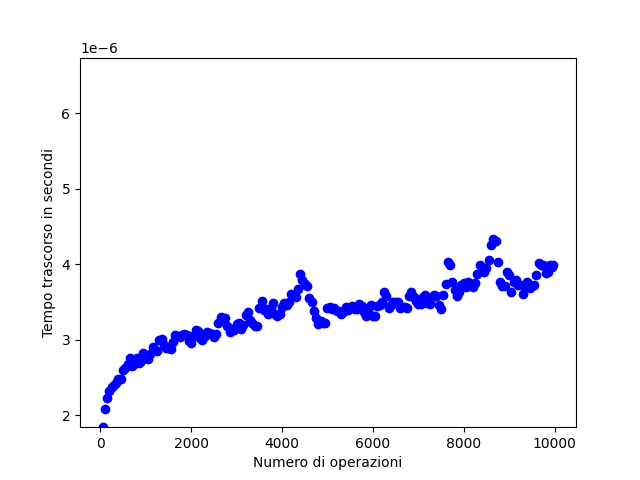
\includegraphics[scale = 0.8]{BST_Deletions}
				\caption{Eliminazioni \textit{input randomizzato}}
			\end{figure}
			\begin{figure}[h!]
				\centering
				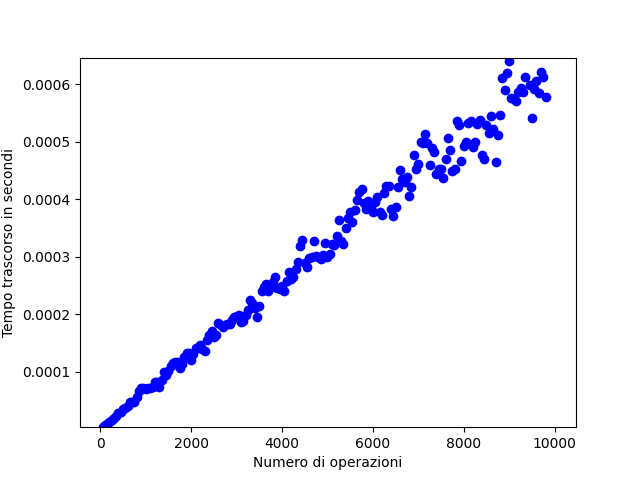
\includegraphics[scale = 0.8]{BST_Unbalanced_Deletions}
				\caption{Eliminazioni \textit{input non bilanciato}}
			\end{figure}
				
		\clearpage
		\subsection{Operazioni su RBT}

			\begin{figure}[h!]
				\centering
				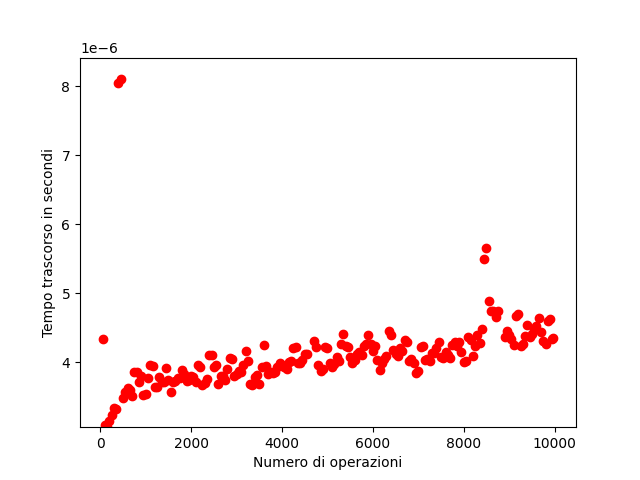
\includegraphics[scale = 0.8]{RBT_Insertions}
				\caption{Inserimenti \textit{input randomizzato}}
			\end{figure}
			\begin{figure}[h!]
				\centering
				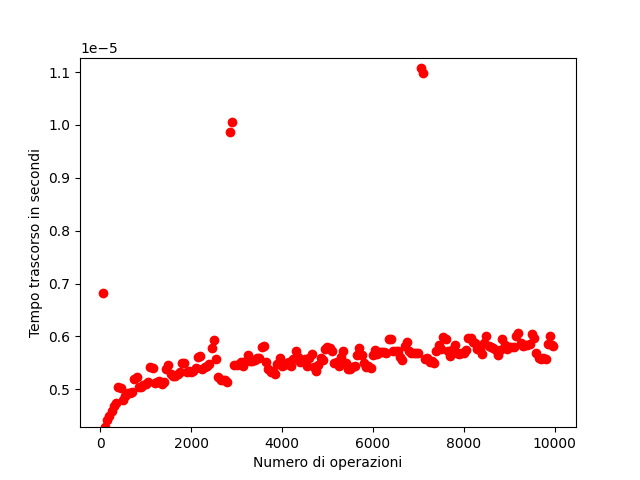
\includegraphics[scale = 0.8]{RBT_Unbalanced_Insertions}
				\caption{Inserimenti \textit{input non bilanciato}}
			\end{figure}
			\begin{figure}[h!]
				\centering
				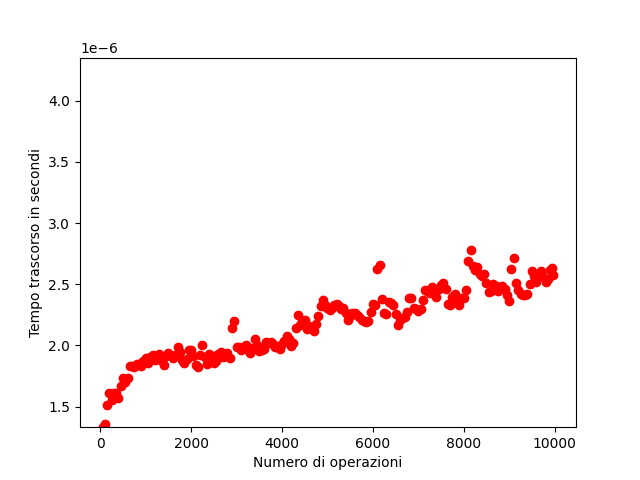
\includegraphics[scale = 0.8]{RBT_Searches}
				\caption{Ricerche \textit{input randomizzato}}
			\end{figure}
			\begin{figure}[h!]
				\centering
				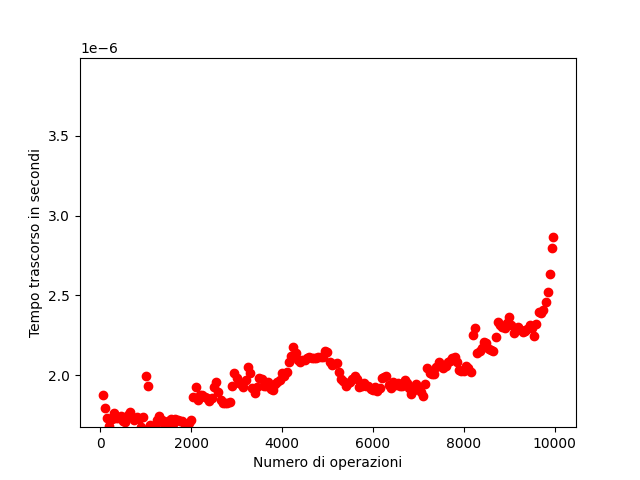
\includegraphics[scale = 0.8]{RBT_Unbalanced_Searches}
				\caption{Ricerche \textit{input non bilanciato}}
			\end{figure}
			\begin{figure}[h!]
				\centering
				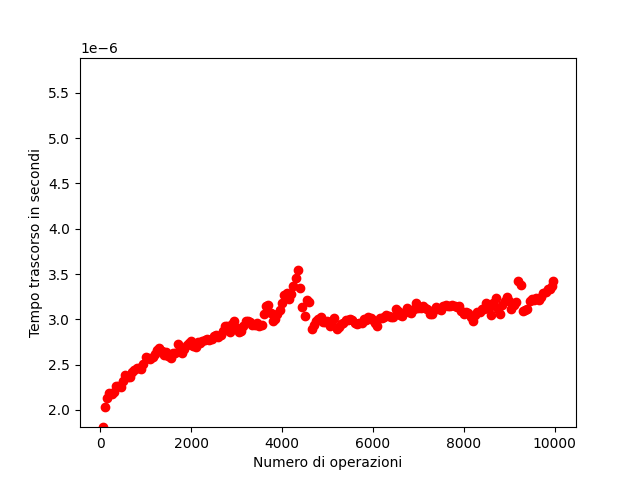
\includegraphics[scale = 0.8]{RBT_Deletions}
				\caption{Eliminazioni \textit{input randomizzato}}
			\end{figure}
			\begin{figure}[h!]
				\centering
				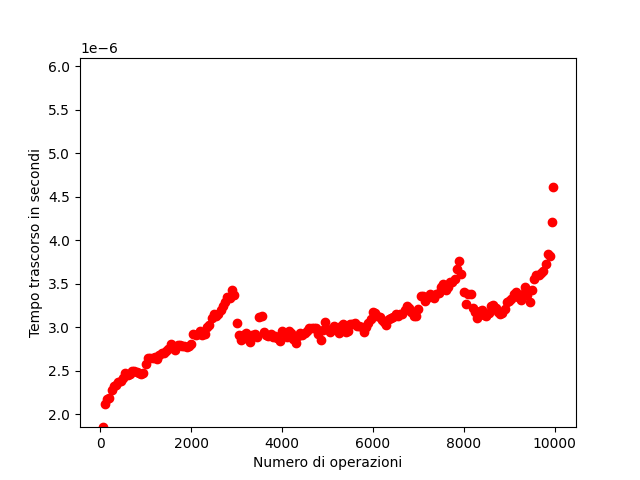
\includegraphics[scale = 0.8]{RBT_Unbalanced_Deletions}
				\caption{Eliminazioni \textit{input non bilanciato}}
			\end{figure}
		
		\clearpage

	\section{Conclusioni}
		I risultati test effettuati coincidono con la complessità attesa delle operazioni di inserimento, ricerca e eliminazione sulle strutture dati BST e RBT.
		

\end{document}